\documentclass[tikz, border=12pt]{standalone}

\usepackage{tabularx}

\newcolumntype{C}{ >{\centering\arraybackslash}>{\columncolor[rgb]{0.95,.95,1}} m{2cm} }
\newcolumntype{D}{ >{\centering\arraybackslash}>{\columncolor[rgb]{0.95,.95,1}} m{4cm} }
\newcolumntype{E}{ >{\centering\arraybackslash} m{3cm} }

\begin{document}
    
\end{document}
\begin{tabular}{|C|D|E|} \hline 
\rowcolor[rgb]{0.9,1,0.9}
Inequality & Number Line & Interval Notation \\ \hline \hline
$a\leq x \leq b$ & 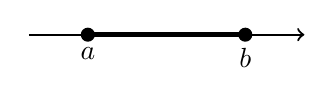
\begin{tikzpicture}[baseline=0.05ex,scale=0.5]
\draw[thick,->] (-3.5,0) -- (3.5,0);
\draw [thick] (-2 cm,2pt) -- (-2 cm,-2pt) node[below] {$a$};
\draw [thick] (2 cm,2pt) -- (2 cm,-2pt) node[below] {$b$};
\draw [line width = 2pt](-2,0) -- (2,0);
\draw [fill=black,thick] (-2,0) circle [radius=0.15];
\draw [fill=black,thick] (2,0) circle [radius=0.15];
\end{tikzpicture} & \onslide<2->{\handout{\white}{}$\displaystyle [a,b]\white|$} \\ \hline

$a\leq x < b$ & 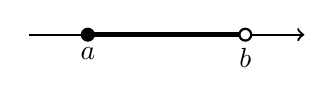
\begin{tikzpicture}[baseline=0.05ex,scale=0.5]
\draw[thick,->] (-3.5,0) -- (3.5,0);
\draw [thick] (-2 cm,2pt) -- (-2 cm,-2pt) node[below] {$a$};
\draw [thick] (2 cm,2pt) -- (2 cm,-2pt) node[below] {$b$};
\draw [line width = 2pt](-2,0) -- (2,0);
\draw [fill=black,thick] (-2,0) circle [radius=0.15];
\draw [fill=white,thick] (2,0) circle [radius=0.15];
\end{tikzpicture}  & \onslide<3->{\handout{\white}{}$\displaystyle [a,b)\white|$} \\ \hline

$a < x \leq b$ & 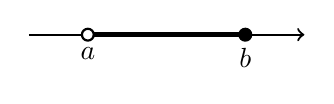
\begin{tikzpicture}[baseline=0.05ex,scale=0.5]
\draw[thick,->] (-3.5,0) -- (3.5,0);
\draw [thick] (-2 cm,2pt) -- (-2 cm,-2pt) node[below] {$a$};
\draw [thick] (2 cm,2pt) -- (2 cm,-2pt) node[below] {$b$};
\draw [line width = 2pt](-2,0) -- (2,0);
\draw [fill=white,thick] (-2,0) circle [radius=0.15];
\draw [fill=black,thick] (2,0) circle [radius=0.15];
\end{tikzpicture}  & \onslide<4->{\handout{\white}{}$\displaystyle (a,b]\white|$} \\ \hline

$a < x < b$ & 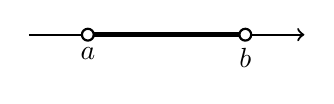
\begin{tikzpicture}[baseline=0.05ex,scale=0.5]
\draw[thick,->] (-3.5,0) -- (3.5,0);
\draw [thick] (-2 cm,2pt) -- (-2 cm,-2pt) node[below] {$a$};
\draw [thick] (2 cm,2pt) -- (2 cm,-2pt) node[below] {$b$};
\draw [line width = 2pt](-2,0) -- (2,0);
\draw [fill=white,thick] (-2,0) circle [radius=0.15];
\draw [fill=white,thick] (2,0) circle [radius=0.15];
\end{tikzpicture} & \onslide<5->{\handout{\white}{}$\displaystyle (a,b)\white|$}  \\ \hline

$a \leq x $ & 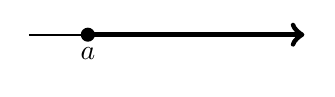
\begin{tikzpicture}[baseline=0.05ex,scale=0.5]
\draw[thick] (-3.5,0) -- (3.5,0);
\draw [thick] (-2 cm,2pt) -- (-2 cm,-2pt) node[below] {$a$};
\draw [line width = 2pt,->](-2,0) -- (3.5,0);
\draw [fill=black,thick] (-2,0) circle [radius=0.15];
\end{tikzpicture} & \onslide<6->{\handout{\white}{}$\displaystyle [a,\infty)\white|$} \\ \hline

$a < x $ & 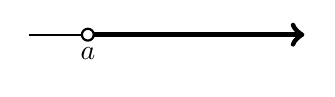
\begin{tikzpicture}[baseline=0.05ex,scale=0.5]
\draw[thick] (-3.5,0) -- (3.5,0);
\draw [thick] (-2 cm,2pt) -- (-2 cm,-2pt) node[below] {$a$};
\draw [line width = 2pt,->](-2,0) -- (3.5,0);
\draw [fill=white,thick] (-2,0) circle [radius=0.15];
\end{tikzpicture} & \onslide<7->{\handout{\white}{}$\displaystyle (a,\infty)\white|$} \\ \hline

$x \leq b$ & 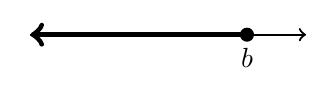
\begin{tikzpicture}[baseline=0.05ex,scale=0.5]
\draw[thick,->] (-3.5,0) -- (3.5,0);
\draw [thick] (2 cm,2pt) -- (2 cm,-2pt) node[below] {$b$};
\draw [line width = 2pt,<-](-3.5,0) -- (2,0);
\draw [fill=black,thick] (2,0) circle [radius=0.15];
\end{tikzpicture}  & \onslide<8->{\handout{\white}{}$\displaystyle (-\infty,b]\white|$} \\ \hline

$x < b$ & 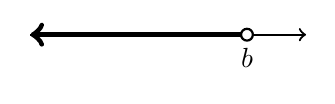
\begin{tikzpicture}[baseline=0.05ex,scale=0.5]
\draw[thick,->] (-3.5,0) -- (3.5,0);
\draw [thick] (2 cm,2pt) -- (2 cm,-2pt) node[below] {$b$};
\draw [line width = 2pt,<-](-3.5,0) -- (2,0);
\draw [fill=white,thick] (2,0) circle [radius=0.15];
\end{tikzpicture} & \onslide<9->{\handout{\white}{}$\displaystyle (-\infty,b)\white|$}  \\ \hline

\end{tabular}

\end{document}